\section{Grundlagen}
\begin{frame}{}
    \begin{center}
        Grundlagen
     \end{center}
\end{frame}

\begin{frame}{Ein typisches Freifunk Netz}
    \begin{itemize}
        \item Ein Batman-Adv Netz
        \begin{itemize}
            \item[$\rightarrow$] "Wie ein großer dezentraler Switch"
        \end{itemize}
        \item VPN (fastd) für die Funkinseln
        \begin{itemize}
            \item Multi-Client zu Multi-Client VPN
            \item Kein internes Routing
            \item Kein Forwarding
            \item Layer-II Netz
        \end{itemize}
        \item Mehrere VPN Server / Gateway
        \begin{itemize}
            \item DHCP
            \item DNS Namensauflösung
            \item Gateway zum Internet / ICVPN
            \begin{itemize}
                \item \zb{} mittels Policy-based routing
            \end{itemize}
        \end{itemize}
        \item Monitoring
        \begin{itemize}
            \item Karte aller Knoten
        \end{itemize}
    \end{itemize}
\end{frame}

\begin{frame}{Freifunk Router (aussen)}
    \begin{itemize}
        \item Client-Ports \& Infrastructure Funknetz:
            Wie ein großer Switch
        \item Batman-Ports \& Ad-Hoc Funknetz:
            Mesh-Netz
        \item WAN-Ports:
            VPN Netz
    \end{itemize}
    \center{
        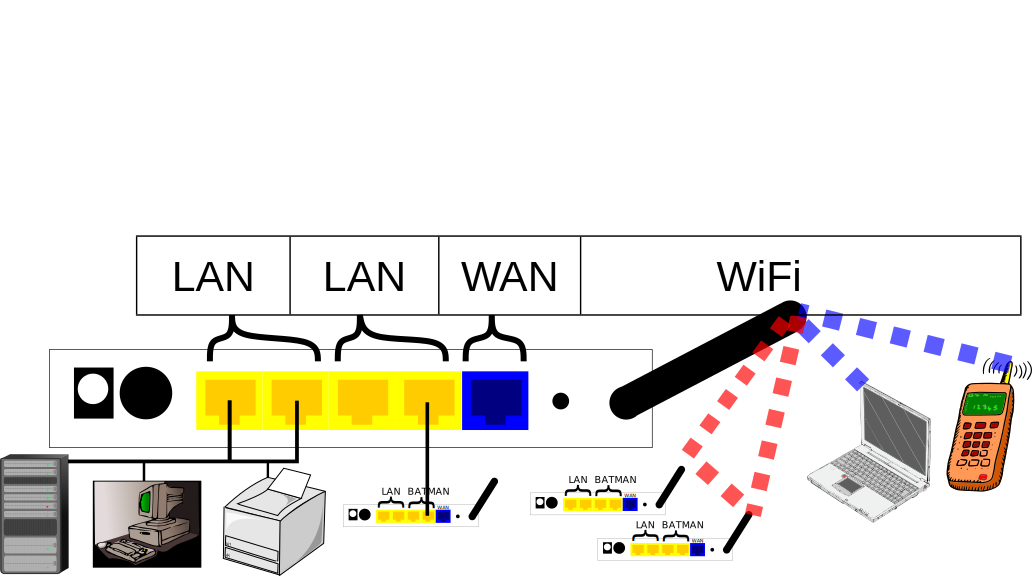
\includegraphics[width=0.75\textwidth]{img/svg/anschluesse.pdf}
    }
\end{frame}

\begin{frame}{Freifunk Router (innen)}
    \begin{itemize}
        \item OpenWrt
        \item Batman-Adv
        \item Fastd Client
        \item Monitoring Daten (Nodewatcher / Alfred)
        \item .. kleinere Tools / Configs / Skripte
    \end{itemize}

    \renewcommand{\arraystretch}{1.5}
    \begin{tabular}{|c|c|c|c|c|c|c|} \hline
         \multicolumn{7}{|c|}{Bridge} \\ \hline
         \multirow{2}{*}{Managed} &
         \multicolumn{4}{c|}{B.A.T.M.A.N} &
         \multicolumn{2}{c|}{\multirow{2}{*}{Client-VLan}} \\ \cline{2-5}
         & Ad-Hoc & VPN & \multicolumn{2}{c|}{Node-VLan} & \multicolumn{2}{c|}{} \\ \hline
         \multicolumn{2}{|c|}{WiFi} & WAN & LAN1 & LAN2 &
         LAN3 & LAN4 \\ \hline
    \end{tabular}
\end{frame}

\begin{frame}{Ein typisches Freifunk Netz}
    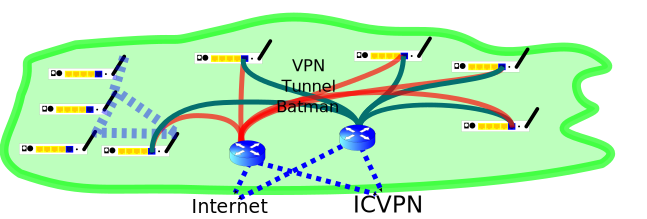
\includegraphics[width=\textwidth]{img/svg/freifunk_konzepte_alt.pdf}
\end{frame}

\begin{frame}{Freifunk Franken Netz}
    \includegraphics[width=\textwidth]{img/svg/freifunk_konzepte.pdf}

    \begin{itemize}
        \item Mehrere Layer-2 Inseln (Hoods)
        \item Verbindung per Layer-3
        \item Dezentrale Gateways
    \end{itemize}
\end{frame}
